\section{Discussion}
In this chapter we have shown at length how to implement event-driven ABS in a pure functional way. We built on the concepts developed in the previous Chapter \ref{ch:timedriven} on time-driven ABS and substantially extended them by various new concepts, necessary for an event-driven approach. Throughout this chapter it became clear that an event-driven approach relies much more on side-effect than a time-driven one and thus requires the sequential update strategy, as side-effects always impose an ordering of execution.

Transforming a time-driven into an event-driven approach should always be possible because the ability to schedule events with timestamps allows to map all features of time-driven ABS to an event-driven one. The process of turning the time-driven SIR into an event-driven one should give a good direction of how this works. Still for some models one can argue that the time-driven approach is much more expressive than an event-driven one, and we think this is certainly the case for the SIR model. The event-driven approach leads to a quite fragmented logical flow and agent behaviour especially in the case of synchronous agent interactions. Still, we have shown a possible direction of reducing the fragmentation using the \textit{tagless final} approach.

\subsection{A Related Approach}
The work of \cite{botta_time_2010} tries to solve a similar problem as we do in this chapter. The authors also use Haskell to implement ABS, and more specifically, look into the use of messages and the problem of when to advance time in models with an arbitrary number of synchronised agent interactions.
The biggest difference is that we approach our agents fundamentally differently through the use of Monads and FRP. In our approach an agent is only a single \texttt{MSF} and thus can not be directly queried for its internal state, its id or outgoing messages. Instead of taking a list of messages, our agents take a single event and can produce an arbitrary number of outgoing events together with an observable state. This would allow us to query the agent for its id and its state by simply sending a corresponding event to the agents MSF and let the agent handle it. Additionally, the state of our agents is \textit{completely} localised and there is no means of accessing the state from outside the agent, they are thus 'fully encapsulated agents' \cite{botta_time_2010}. The authors define their agents with a polymorphic agent-state type \texttt{s}, which implies that without knowledge of the specific type of \texttt{s} there would be no way of accessing the state, rendering it also fully encapsulated.
The problem of advancing time in our approach is conceptually very similar. After sending a \texttt{Tick} message to each agent in random order, we process all agents until they are idle and there are no more enqueued events in the list. %The similarities in both approaches might hint at that this seems to be indeed the 'right' way to go.

\subsection{Layered architecture}
Our approach is designed as a triple layered architecture, see Figure \ref{fig:3layer_system}:
\begin{enumerate}
	\item \textit{Pure Functions} are the work horses that do the actual computations of the simulation. They are mostly used to build up the 2nd layer. Additionally, layer 3 might access them to achieve pure computations when there is no need for effects.
	
	\item \textit{Monad Transformer Stack} (global and local) does the 'dirty' work of effectful computation: sending messages, mutating the environment, reading model configuration, drawing random numbers, mutating agent state. This layer uses the pure functions to build up its functionality and also propagates between the 1st and 3rd layer.
	
	\item \textit{MSF} is the backbone of the architecture and defines the dynamical structure of the system. This layer builds heavily on the 2nd layer and can also be seen as a high-level delegation mechanism.
\end{enumerate}

\begin{figure}
	\centering
	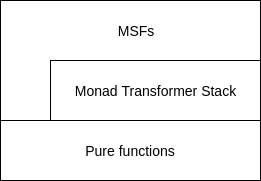
\includegraphics[width=.4\textwidth, angle=0]{./fig/eventdriven/3layers.png}
	\caption[Three layered architecture of event-driven ABS]{Three layered architecture of event-driven ABS.}
	\label{fig:3layer_system}
\end{figure}

Separating those three concerns from each other makes the code more robust, easier to refactor and maintain. Further it makes code \textit{much} easier to test as will be shown in Chapter \ref{ch:property}. 

\subsection{Imperative Nature}
Both event-driven use cases make heavy use of the \texttt{State} Monad, thus one might ask what the benefits are of our pure functional approach, after all, we seem to fall back into stateful, imperative style of programming.
The crucial point is that it is highly restricted to very specific types and operations. In the Monad stack we control the operations possible in to the respective layers, for example sending events is a write-only operation, accessing the unique agent id and the model configuration is read only. All this is guaranteed at compile time, which makes it much more manageable, maintainable, robust, composable and testable.
To quote \href{https://www.gamasutra.com/view/news/169296/Indepth_Functional_programming_in_C.php}{John Carmack}~\cite{gamasutra_carmack_fp}: \emph{"A large fraction of the flaws in software development are due to programmers not fully understanding all the possible states their code may execute in."}. We claim that despite using an imperative style, the static guarantees of the types we operate on and the operations provided, make it easier to fully understand the possible states of the simulation code.
This is directly related to the power of polymorphism in Haskell, which goes far beyond the polymorphism of existing object-oriented \footnote{Polymorphism is \textit{not} unique to object-oriented programming.} languages.
We see a particular instance of that in the polymorphism we developed in the concepts behind Sugarscape where we can compose effects depending on the model and we can easily swap out environment and events with very few changes with the benefit that the compiler will inform us about breaking changes. This is directly related to refactoring, which is very convenient and quickly becomes the standard in the development process. Guided by defining types first and relying on the compiler to point out problems, results in very effective and quick changes without danger of bugs showing up at run time. This is not possible in dynamic object-oriented languages like Python because of its lack of a compiler and types, and is also much less effective in Java which is only remedied through strong IDE support.

\subsection{Handling IO}
This thesis directly capitalises on the fact that most ABS models are primarily of computational nature, thus CPU bound, not involving \texttt{IO} \textit{inside the agents} while running the simulation. The concurrent approach with Software Transactional Memory in Chapter \ref{ch:concurrent_abs} is an exception but at least we retain the guarantees that the non-determinism within the agent behaviour originates from the concurrency using Software Transactional Memory and nothing else. Even if some \texttt{IO} is required, like rendering the simulation as we did in Sugarscape, due to the loose coupling and compositional qualities of pure functional programming it is straightforward to separate these concerns and keep the impure rendering parts from the pure agent behaviour.

If there arises the use case where agents absolutely need to perform some impure IO within their behaviour, then there are three options. The first one is to let agents construct \texttt{IO} actions and pass them to the simulation kernel for execution, requiring the simulation kernel to run now in \texttt{IO} instead of being pure. This is especially suitable for one-way \texttt{IO} actions, where an agent does not need to synchronously wait for a result. If a synchronous \texttt{IO} action is required with the agent waiting for a result, it could be communicated back from the simulation kernel. This keeps the agent behaviour still pure, but with the consequence of indirection and higher complexity. The second option is to use a \textit{tagless final} approach as discussed in Chapter \ref{sec:tagless_final_basics}, where the actions requiring IO are abstracted behind methods of the given type class, for which then an interpreter running in \texttt{IO} has to be written. The benefit is that this allows for direct synchronous IO behaviour, while still restricting the available operations to only the required ones instead of running fully in the \texttt{IO} Monad as would be the third option. In all cases everything becomes possible and all bets are off regarding static guarantees and reproducibility, whereas the tagless final approach provides the most control.

\subsection{Multiple types of Agents}
In the Sugarscape example we have only considered one type of agents, thus the whole population is a homogeneous one in regards of the \textit{type} of the agent. It is quite straightforward to have heterogeneous agent types as well, which is accomplished through adding additional data declarations to the observable output and the agent state. A consequence is that all agent types have to speak the same event language because in regards of types the agents are treated the same way. This is also true for the monadic stack where different agent types cannot have different effect types in this approach as they are seen as the same on the type level.

\subsection{Performance}
\label{sub:eventdriven_performance}
The event-driven implementation from this Chapter is around 60 - 70\% faster than the time-driven implementation from Chapter \ref{sec:timedriven_firststep}, which is non-monadic and uses the FRP library Yampa. For the monadic time-driven approach of Chapter \ref{sec:adding_env} the difference is much more dramatic as it is about 700 - 800\% faster. These results dramatically highlight the problem of time-driven ABS and shows that its performance cannot compete with an event-driven approach. This situation is exaggerated even more so when making use of MSFs as in Chapter \ref{sec:adding_env}. In this case, a time-driven approach becomes extremely expensive in terms of performance and one should consider an event-driven approach. In case the model is specified in a time-driven way, a transformation into an event-driven approach should always be possible as outlined above.

We compared an event-driven SIR implementation we did in Java to the Haskell one here. We run for 150 time steps with 1,000 susceptible and 1 infected agent, $\beta = \frac{1}{5}$, $\gamma = 0.05$, $\delta = 15$. Further, we fixed the random number generators to guarantee identical dynamics in every run and averaged 8 runs. The Java implementation averages at 1.2 seconds, whereas the Haskell implementation at 6.8 seconds. These performance figures are closer than the ones in the time-driven approach of the previous chapter. This shows that event-driven indeed performs much better and is also more flexible as \cite{meyer_event-driven_2014} has pointed out. Curiously, the \textit{time-driven} Java implementation outperforms the event-driven Java one. Although, we have improved the performance substantially compared to the time-driven approach, we address it more in depth in the Chapter \ref{ch:parallelism_ABS} on parallelism and Chapter \ref{ch:concurrent_abs} on concurrency.

% EVENT-DRIVEN
% Java: 1262, 1259, 1159, 1202, 1182, 1152, 1238, 1238 Milliseconds
% Haskell: 6.8, 6.6, 6.3, 6.3, 6.5, 6.3, 6.3, 6.8 Seconds

\subsection{Conclusion}
Overall we think that this event-driven approach is quite feasible and is \textit{the way to go} to implement ABS in a pure functional way. The time-driven approach is quite expressive but is not as flexible and general as the event-driven one. Additionally the performance is considerably better in an event-driven approach.

We conclude that synchronous agent interaction is the most difficult part to figure out and get right and thus poses the greatest challenge. This concept is indeed cumbersome and clearly more complex than direct method invocation in object-oriented programming. Unfortunately, with the goal of staying pure we do not have much other options. We didn't aim to encapsulate its complexity behind domain-specific combinators, but this is certainly possible and should reduce the difficulty and complexity considerably. This is left for further research and open work which should be undertaken in the future, when putting all the concepts of this thesis into a general purpose library for pure functional ABS in Haskell.